\documentclass{article}
\usepackage{amsmath,amsthm,amssymb}
\usepackage{graphicx}
\newcommand{\version}{atlas ver. 0.2, Apr 30 2012}

\title{Cartography of a 4-dimensional flow: A visual guide to sections and slices}
\author{Daniel Borrero-Echeverry, Keith M. Carroll,Bryce Robbins,\\ Evangelos Siminos and Lei Zhang}
\date{\today}
\begin{document}

\maketitle





    \begin{abstract}

We provide method of slice as a way to quotient the continuous symmetries of chaotic flows. The basic idea is to use a set of hyperplanes (called charts), each covering a neighbourhood of a dynamically important solutions (a 'template'). All the charts together provide an atlas for the symmetry reduced state space, which charted the regions explored by the trajectories of interest. By slicing, relative equilibria reduce to equilibria and relative periodic orbits reduce to periodic orbits. Visualizations of these solutinos and their unstable manifolds reveal their interrelations and the role they play in organizing turbulence/chaos.

    \end{abstract}



    \begin{quotation}
Today, it is possible to take a stroll through 61,506 dimensional state spae of hydrodynamic turbulence. Charting this world is a geometer's task, and we will map it using a measuring tape, but first one has to deal with symmetries. Physicists have come to love them inordinately, but Nature less so: even though the governing equations are symmetric, turbulence breaks all symmetries, and for nonlinear systems, rather than simplifying our task, symmetries obscure the essential dynamics. While evolution in time decomposes the state space into a spaghetti of time trajectories, continuous spatial symmetries stratify it like the layers of an onion. In this tangle and pick a single representative point for each trajectory (section it) and group orbit (slice it). Once the fog of symmetries is out of the way, one can identify and describe the prominent fluid structures by a taxonomy of its invariant building blocks: numerically exact solutions of Navier-Stokes equations, finite sets of relative equilibria and infinite hierarchies of relative periodic orbits, and describe the dynamics in terms of their heteroclinic connections.
    \end{quotation}

\section{Introduction}
\label{s:intro}

Over the last decade, new insights into the dynamics of  [blah blah]

Our goals here are ?-fold:
(i)  [blah blah].
(ii) [blah blah].

we shall illustrate the key ideas by a much
simpler example, the $SO(2)$-equivariant  [blah blah],

\section{Section}
\label{s:cut}


As an example consider the  [blah blah],

%%%%%%%%%%%%%%%%%%%%%%%%%%%%%%%%%%%%%%%%%%%%%%%%%%%%%%%%%%%%%%%%%%%%%
%%\begin{figure}
%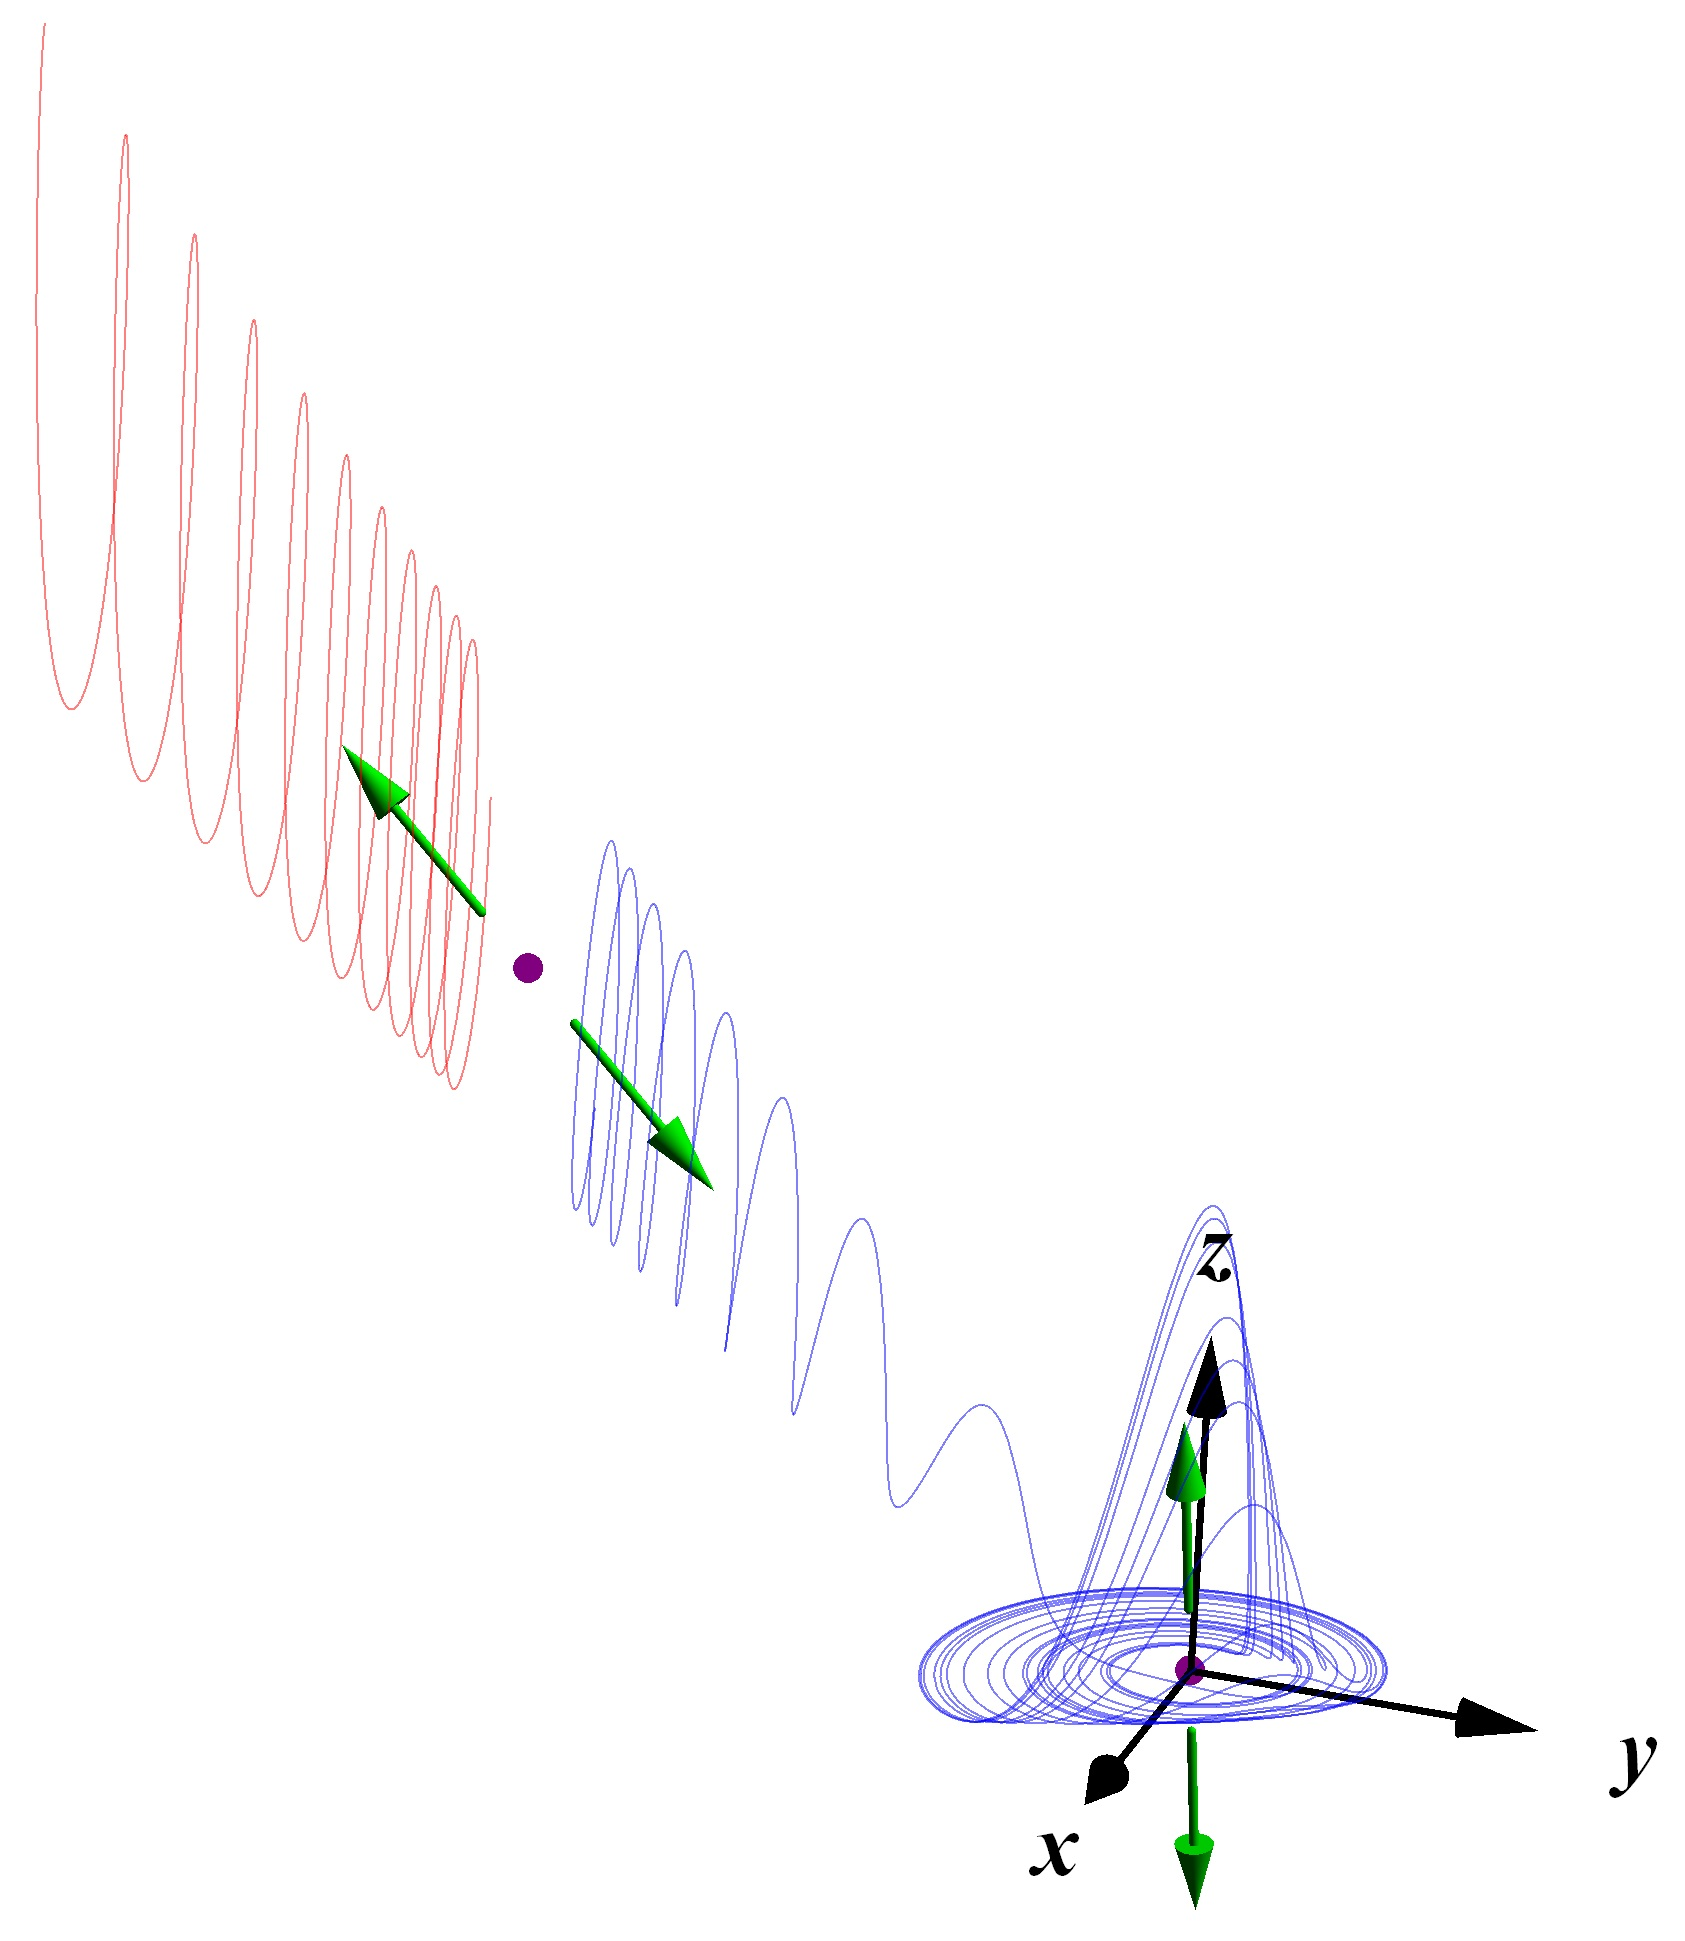
\includegraphics[width=0.28\textwidth]{RoessTrjs2}%{Rossler_Equilibria2}{RoessTrjs}%
%% \begin{center}
%% \setlength{\unitlength}{0.20\textwidth}
%%(a)
%%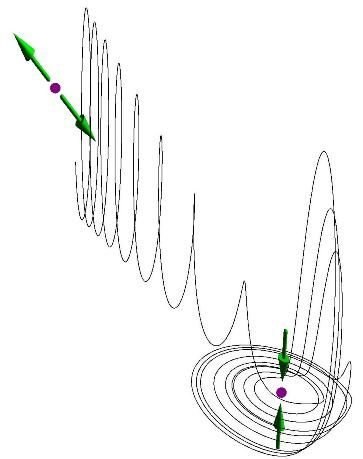
\includegraphics[width=\unitlength,clip=true]{RoessTrajLbld2}
%%(b)
%%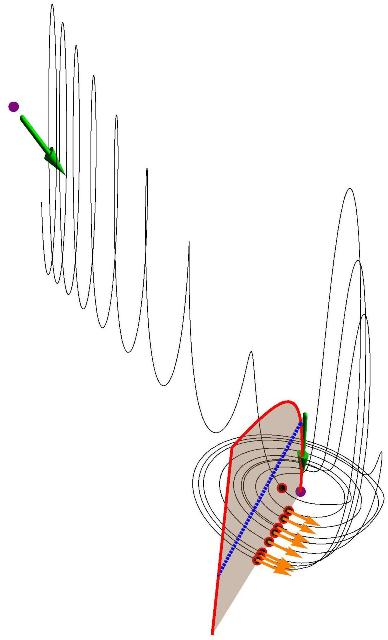
\includegraphics[width=\unitlength,clip=true]{RoessNeareqLbld2}
%%\\
%%(c) 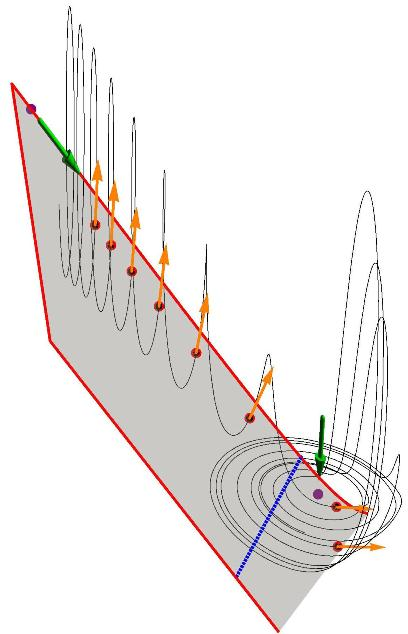
\includegraphics[width=\unitlength,clip=true]{RoessFareqLbld2}
%%(d) 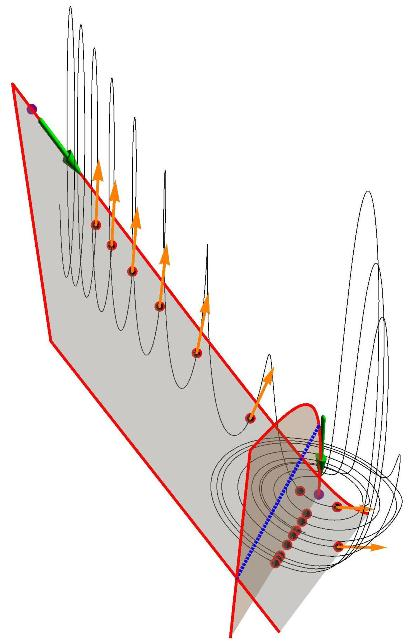
\includegraphics[width=\unitlength,clip=true]{RoessBotheqLbld2}
%% \end{center}
%%    \caption{
%%2-chart atlas for Porter-Knobloch\ flow.
%%(a)
%%(b)
%%(c)
%%(d)
%%    }
%%\label{fig:2modeSects}
%%\end{figure}
%%%%%%%%%%%%%%%%%%%%%%%%%%%%%%%%%%%%%%%%%%%%%%%%%%%%%%%%%%%%%%%%%%%%%

 [blah blah]

\section{Dynamics and symmetry}
\label{s:symm}

\subsection{Porter-Knobloch $SO(2)$-equivariant flow}
\label{s:twoMode}

We consider a system constructed from Fourier modes $(m,n)$\ref{Dang86,AGHO288,PoKno05}, which is invariant under symmetry group $SO(2)$ as rotation
\begin{equation}
(z_1,z_2)\to(e^{mi\phi}z_1,e^{ni\phi}z_2)\label{Dang86(1.1)aa}
\end{equation}
We will only consider the case with Fourier mode (1,2). For this system, the basis for $SO(2)$ invariant polynomials are
\begin{align}
u&=z_1\bar{z_1}\\
v&=z_2\bar{z_2}\\
w&=z_1^2\bar{z_2}+\bar{z_1}^2z_2\\
q&=(z_1^2\bar{z_2}-\bar{z_1^2}z_2)/i\\
\label{Dang86(1.2)PK}
\end{align}

In polar coordinates
\begin{equation}
z_1=|u|^{1/2}e^{i\theta_1}
z_2=|v|^{1/2}e^{i\theta_2}
\end{equation}
we can write the invaraint polynomials as
\begin{align}
w=2\Re(z_1^2\bar{z_2})=2u|v|^{1/2}\cos\psi\\
q=2\Im(z_1^2\bar{z_2})=2u|v|^{1/2}\sin\psi
\label{Dang86(1.2)polar}
\end{align}
where $\psi=2\theta_1-\theta_2$



 The polynomials $\{u,v,w,q\}$ are
linearly independent, but related through one syzygy,
\begin{equation}
w^2+q^2 - 4\,u^2v =0
\label{eq:syzPK}
\end{equation}
confining the dynamics to a 3-dim\-ens\-ion\-al $\mathcal{M}/SO(2)$ reduced state space
manifold, a symmetry-invariant repre\-sent\-ati\-on of the 4-dim\-ens\-ion\-al
$SO(2)$ equivariant dynamics.

Substitute ${z_1,\bar{z}_1,z_2,\bar{z}_2}$ with ${u,v,w,q}$ and apply chain rule
\( %beq
 \dot{ u}_i= ({\partial u_i}/{\partial x_j}) \, \dot{x}_j
 \,,
\) %ee{HilbChainRl}
we get
\begin{align}
  \dot{u} &=\overline{z}_1 \dot{z}_1 + {z}_1 \dot{\overline{z}}_1\\
  \dot{v} &= \overline{z}_2 \dot{z}_2 + {z}_2 \dot{\overline{z}}_2\\
  \dot{w} &= 2 \,\overline{z}_2 {z}_1 \dot{z}_1
           + 2\,{z}_2 \overline{z}_1 \dot{\overline{z}}_1
           + {z}_1^2 \dot{\overline{z}}_2
           + \overline{z}_1^2 \dot{z}_2\\
  \dot{q} &=  (2\,\overline{z}_2 {z}_1 \dot{z}_1
           - 2\,{z}_2 \overline{z}_1 \dot{\overline{z}}_1
           + {z}_1^2 \dot{\overline{z}}_2
           - \overline{z}_1^2 \dot{z}_2
           )/i
\label{PKinvEqs}
\end{align}

Dangelmayr,\ref{Dang86} Armbruster, Guckenheimer and Holmes,\ref{AGHO288}
Jones and Proctor,\ref{JoPro87} and Porter and Knobloch\ref{PoKno05} (see
Golubitsky et al\ref{golubII}, Sect. XX.1) have investigated bifurcations
in 1:2 resonance ODE normal form models to third order in the amplitudes.
We shall use here such a model,
\begin{subequations}\label{eq:DangSO2}
\begin{align}
  \dot{z}_1 &= \mu_1\,z_1+a_1\,z_1|z_1|^2+b_1\,z_1|z_2|^2+c_1\,\overline{z}_1\,z_2\,\\
  \dot{z}_2 &= (\mu_2-i\, e_2)\,{z_2}+a_2\,z_2|z_1|^2+b_2\,z_2|z_2|^2+c_2\,z_1^2
\end{align}
\end{subequations}
with complex variables and real parameters. For parameters
far from bifurcation values the model has no physical motivation; in
particular, we introduce the parameter $e_2$ to reduce the $O(2)$ symmetry to $SO(2)$ symmetry. We use it purely to compare and
illustrate different symmetry reduction methods, in the dimensionally
lowest possible setting: a state space of dimension $d=4$, with the
$SO(2)$-reduced dynamics taking place in 3 dimensions, the lowest
possible if the dynamics is to be chaotic. We shall refer to
\ref{eq:DangSO2} as the Porter-Knobloch system, which is a special case $(\omega_1=0)$ for the system considered in \ref{}.The correspondence of parameters are

\begin{align}
\mu_1&\leftrightarrow\mu_1\\
\alpha_r&\leftrightarrow c_1\\
d_{11}&\leftrightarrow a_1\\
d_{12}&\leftrightarrow b_1\\
\mu_2&\leftrightarrow\mu_2\\
\epsilon\omega_2&\leftrightarrow-e_2\\
\beta_r&\leftrightarrow c_2\\
d_{21}&\leftrightarrow a_2 \\
d_{22}&\leftrightarrow b_2
\end{align}
Substituting
\ref{eq:DangSO2} into \ref{PKinvEqs} we obtain a set of 4 equations,
\begin{equation}
\begin{split}
  \dot{u} &= 2\,\mu_1\,u+2\,a_1\,u^2+2\,b_1\,u\,v+c_1\,w\\
  \dot{v} &= 2\,\mu_2\,v+2\,a_2\,u\,v+2\,b_2\,v^2+c_2\,w\\
  \dot{w} &= (2\,\mu_1+\mu_2)\,w+(2a_1+a_2)\,u\,w+(2b_1+b_2)\,v\,w\\
	&+4c_1\,u\,v + 2c_2\,u^2 - e_2\,q
\label{PKinvEqs1}\\
  \dot{q} &= (2\mu_1+\mu_2)\,q+(2a_1+a_2)\,u\,q+(2b_1+b_2)\,v\,q
             +e_2\,w
\end{split}
\end{equation}
One can now either investigate the dynamics in this invariant basis or
plot the `image'\ref{GL-Gil07b} of solutions computed in the equivariant
basis \ref{eq:DangSO2} in terms of these invariant polynomials.


Written the complex Porter-Knobloch system in real variables by substituting $z_1 = x_1 + i x_2$ and $z_2 = y_1 + i y_2$.We rewrirren\ref{eq:DangSO2} as a 4-dimensional first order ODE system			
			\begin{align}
				\dot{x}_1 &= a_1 x_1^3 + b_1 x_1 y_1^2 + c_1 x_1 y_1 + a_1 x_1 x_2^2 + b_1 x_1 y_2^2 + \mu_1 x_1 + c_1 x_2 y_2\\
				\dot{y}_1 &= a_1 x_1^2 x_2 + c_1 x_1 y_2 + b_1 y_1^2 x_2 - c_1 y_1 x_2 + a_1 x_2^3 + b_1 x_2 y_2^2 + \mu_1 x_2\\
				\dot{x}_2 &= a_2 x_1^2 y_1 + c_2 x_1^2 + b_2 y_1^3 + a_2 y_1 x_2^2 + b_2 y_1 y_2^2 + \mu_2 y_1 - c_2 x_2^2 + e_2 y_2\\
				\dot{y}_2 &= a_2 x_1^2 y_2 + 2 c_2 x_1 x_2 + b_2 y_1^2 y_2 - e_2 y_1 + a_2 x_2^2 y_2 + b_2 y_2^3 + \mu_2 y_2
			\end{align}

the stability matrix ({insert DasBuch eq. ref here, originally eq. 4.3}) A for this 				system is given by the matrix $A=(a_{ij})$, where
\begin{align}
a_{11}&=3 a_1 x_1^2 + b_1 y_1^2 + c_1 y_1 + a_1 x_2^2 + b_1 y_2^2 + \mu_1\\
a_{12}&=c_1 y_2 + 2 a_1 x_1 x_2\\
a_{13}&=c_1 x_1 + 2 b_1 x_1 y_1\\
a_{14}&=c_1 x_2 + 2 b_1 x_1 y_2\\
a_{21}&=c_1 y_2 + 2 a_1 x_1 x_2\\
a_{22}&=a_1 x_1^2 + b_1 y_1^2 - c_1 y_1 + 3 a_1 x_2^2 + b_1 y_2^2 + \mu_1\\
a_{23}&=2 b_1 y_1 x_2 - c_1 x_2\\
a_{24}&=c_1 x_1 + 2 b_1 x_2 y_2\\
a_{31}&=2 c_2 x_1 + 2 a_2 x_1 y_1\\
a_{32}&=2 a_2 y_1 x_2 - 2 c_2 x_2\\
a_{33}&=a_2 x_1^2 + 3 b_2 y_1^2 + a_2 x_2^2 + b_2 y_2^2 + \mu_2\\
a_{34}&=e_2 + 2 b_2 y_1 y_2\\
a_{41}&= 2 c_2 x_2 + 2 a_2 x_1 y_2\\
a_{42}&=2 c_2 x_1 + 2 a_2 x_2 y_2\\
a_{43}&= 2 b_2 y_1 y_2 - e_2\\
a_{44}&=a_2 x_1^2 + b_2 y_1^2 + a_2 x_2^2 + 3 b_2 y_2^2 + \mu_2
\label{{2modeStabMatrix}}
\end{align}

The Porter-Knobloch system is equivariant under infinitesimal $SO(2)$ rotations by substituting the Lie algebra generator
    \begin{equation}
\mathbf{T}  \, =
\left( \begin{array}{cccc}
         0 & 1 & 0 & 0 \\
        -1 & 0 & 0 & 0 \\
         0 & 0 & 0 & 2\\
         0 & 0 & -2 & 0
      \end{array} \right)
\label{{LGTwoMode}}
\end{equation}
and A into the equivariance condition.

We can also write the system in polar coordinates
\begin{align}
\dot{r}_1&=r_1(\mu_1+a_1r_1^2+b_1r_2^2+c_1r_2\cos(\psi))\\
\dot{r}_2&=\mu_2r_2+a_2r_1^2r_2+b_2r_2^3+c_2r_1^2\cos(\psi)\\
\dot{\psi}&=e_2-(c_2\frac{r_1^2}{r_2}+2c_1r_2)\sin(\psi)
\end{align}

In polar coordinates, the stability matrix becomes
\begin{equation}
\left(\begin{array}{ccc}
\mu_1+2a_1r_1^2+b_1r_2^2+c_1r_2\cos\psi & 2b_1r_1r_2+c_1r_1\cos\psi & -c_1r_1r_2\sin\psi\\
2c_2r_1\cos\psi & \mu_2+a_1r_1^2+3b_2r_2^2 & -c_2r_1^2\sin\psi\\
-2c_2\frac{r_1}{r_2}\sin\psi & c_2\frac{r_1^2}{r_2^2}\sin\psi-2c_1\sin\psi & -(c_2\frac{r_1^2}{r_2}+2c_1r_2)\cos\psi
\end{array}\right)
\end{equation}


\begin{figure}
\centering
 (a) 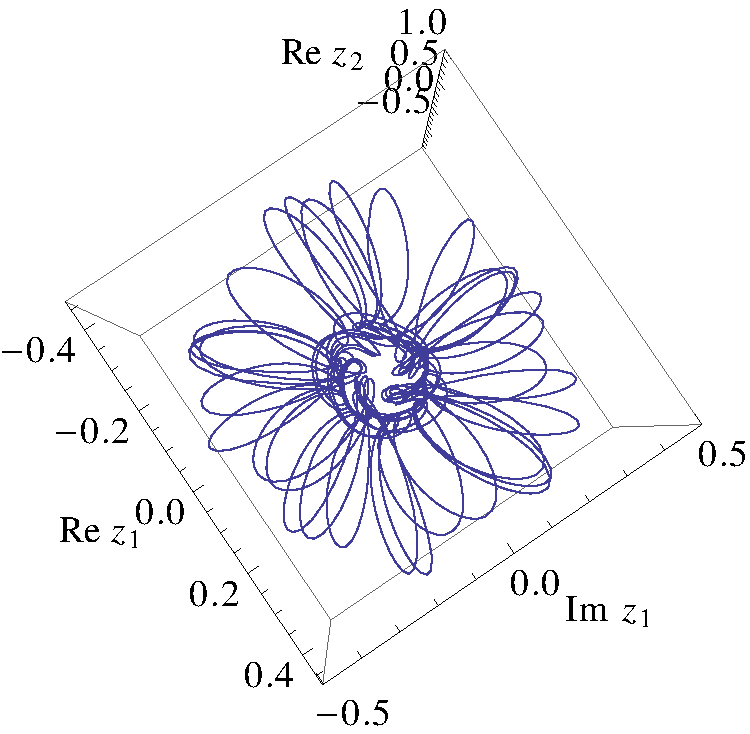
\includegraphics[width=0.35\textwidth]{dangelmayrZ}
 (b) 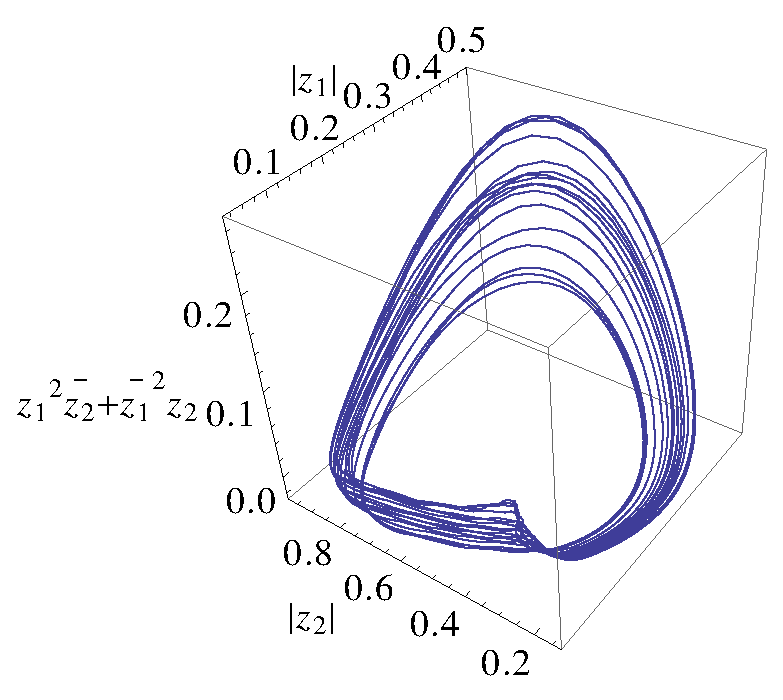
\includegraphics[width=0.35\textwidth]{dangelmayrAGH}
\caption{Projections of Dangelmayr system \ref{eq:DangSO2}
``attractor'' for $\mu_1 = -0.337,\, \mu_2 = 0.27,\, c_1 = 1,\, c_2 =
-1,\, a_1 = -1.5,\, a_2 = -6.19,\, b_1 = 1.583,\,  b_2 = -0.115,\, e_2 =
1.211$
(a) in original state space variables $\Re z_1,\,\Im z_1,\,\Re z_2$.
(b) in invariant coordinates used by
Armbruster et al \ref{AGHO288} $|z_1|,\, |z_2|,\, z_1^2 \bar{z}_2 + \bar{z}_1^2 z_2$.
}
 \label{fig:dangelmayrChaos}
\end{figure}

%%%%%%%%%%%%%%%%%%%%%%%%%%%%%%%%%%%%%%%%%%%%%%%%%%%%%%%%%%%%%%%%%%%%%%%%%%%%%%%%%%%%%%%%%%%%%%%%%%
\subsection{To do}
\label{s:ToDo}

\begin{itemize}

  \item[10.11] Visualizations of the 4-dimensional Porter-Knobloch system
  \item[10.1?] draw a group orbit for the Porter-Knobloch model
  \item[10.23] The relative equilibria of the Porter-Knobloch system
  \item[10.24] Plotting the relative equilibria of
           the Porter-Knobloch system in invariant coordinates
  \item[10.25] Plotting the relative equilibria of
           the Porter-Knobloch system in Cartesian coordinates
  \item[10.2?] construct a 2-chart atlas for a Porter-Knobloch system
\end{itemize}


 [blah blah]

Mercader and Prat\ref{MePrKn01} might
be a candidate if we decide to go with $O(2)$ symmetry since really the
Rayleigh-Benard problem has $O(2) \times Z_2$ symmetry and they are really
talking about breaking the $Z_2$ part.

 [blah blah]


 [blah blah]

\begin{itemize}
  \item $TW_1 = (r_1,r_2,\psi)=(0.0516508, 1.26311,?)$ and
        $TW_2 = (0.467095,0.2146,?)$
  \item their plots in the Cartesian coordinates
  \item $\dot{\theta}$ to see how slow/fast are they. $\dot{\theta}$
        might be related to 4th eigenvalue, when you go back
        to Cartesian coordinates
  \item stability eigenvalues, eigenvectors of the equilibrium $EQ_0$ at
        origin, at your parameter values - if it is stable, everything
        just might fall into it and die.
  \item plots of small perturbations of the above equilibrium and relative equilibrium in
        the Cartesian coordinates to see whether the dynamics looks
        chaotic
  \item $TW_1$: 2 large positive eigenvalues looks scary - probably
        nothing re-visits this relative equilibrium. A mildly unstable complex pair
        would have been sweeter. You get complex eigenvalue by Hopf-bifurcating off a
        stable orbit, typically.
  \item $TW_1$: Does either unstable eigenvalue become a complex
        eigenvalue pair in Cartesian coordinates?
  \item $TW_2$: contracting eigenvalues have very small imaginary
        part, so the presumably just rocket toward the relative equilibrium, not much
        spiraling there. At least the unstable eigenvalue seems slow
        compared to all other eigenvalues.
  \item $TW_1$: Does the unstable eigenvalue become a complex
        eigenvalue pair in Cartesian coordinates?
\end{itemize}

 [blah blah]



%%%%%%%%%%%%%%%%%%%%%%%%%%%%%%%%%%%%%%%%%%%%%%%%%
% 2011-09-09, 2012-03-30 Predrag: add BeThMovFr to
%            continuous.tex overheads, and ChaosBook
% replace A27movFrame*.* everywhere
%\begin{figure}
%  	\begin{center}
%  	\setlength{\unitlength}{0.20\textwidth}
%  (a)
%  	\begin{picture}(1,1.07802818)%
%    	\put(0,0){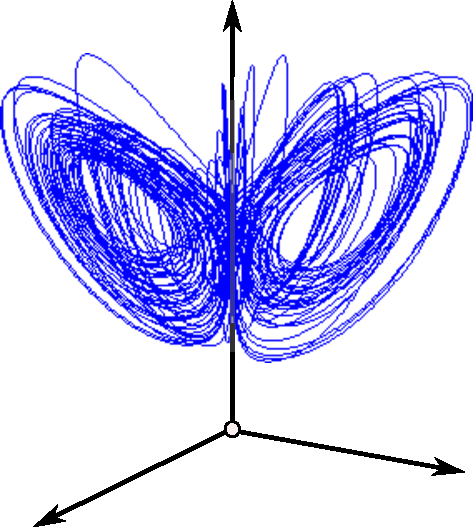
\includegraphics[width=\unitlength]{CLEattractor}}%
%    	\put(0.55152995,1.0139628){\color[rgb]{0,0,0}\makebox(0,0)[lb]{\smash{$z$}}}%
%    	\put(0.05573445,0.0739776){\color[rgb]{0,0,0}\makebox(0,0)[lb]{\smash{$x_1$}}}%
%    	\put(0.90013492,0.16491708){\color[rgb]{0,0,0}\makebox(0,0)[lb]{\smash{$x_2$}}}%
%  	\end{picture}%	
%  (b)
%  	\begin{picture}(1,1.06440474)%
%    	\put(0,0){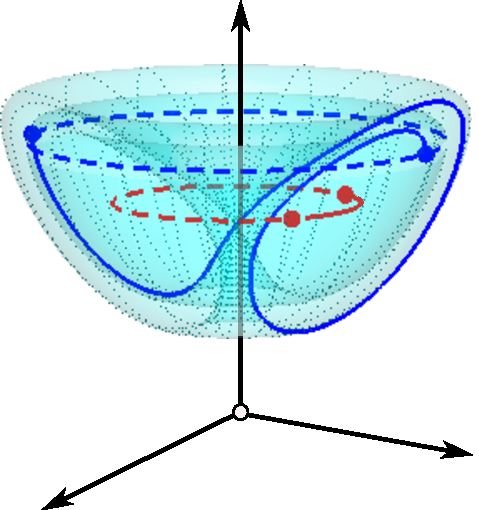
\includegraphics[width=\unitlength]{CLEWurst01}}%
%   		\put(0.55961552,1.00214901){\color[rgb]{0,0,0}\makebox(0,0)[lb]{\smash{$z$}}}%
%   		\put(0.07008555,0.07304272){\color[rgb]{0,0,0}\makebox(0,0)[lb]{\smash{$x_1$}}}%
%    	\put(0.90381504,0.16283301){\color[rgb]{0,0,0}\makebox(0,0)[lb]{\smash{$x_2$}}}%
%  	\end{picture}
%\\
%(c)   \begin{picture}(1,0.94310243)%
%    \put(0,0){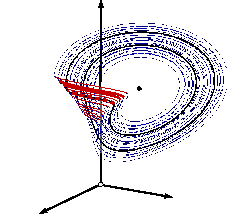
\includegraphics[width=\unitlength]{CLE1SliceSmall.pdf}}%
%    \put(0.48564392,0.89244183){\color[rgb]{0,0,0}\makebox(0,0)[lb]{\smash{$z$}}}%
%    \put(0.07181137,0.03185892){\color[rgb]{0,0,0}\makebox(0,0)[lb]{\smash{$y_2$}}}%
%    \put(0.77031544,0.100183){\color[rgb]{0,0,0}\makebox(0,0)[lb]{\smash{$x_2$}}}%
%  \end{picture}%
%(d)   \begin{picture}(1,1.05662086)%
%    \put(0,0){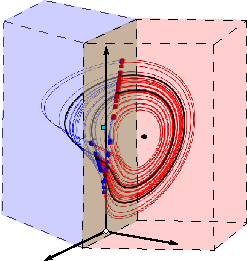
\includegraphics[width=\unitlength]{CLE2slicesmall.pdf}}%
%    \put(0.47706962,0.83002768){\color[rgb]{0,0,0}\makebox(0,0)[lb]{\smash{$z$}}}%
%    \put(0.08719004,0.02997825){\color[rgb]{0,0,0}\makebox(0,0)[lb]{\smash{$y_2$}}}%
%    \put(0.73025395,0.09287946){\color[rgb]{0,0,0}\makebox(0,0)[lb]{\smash{$x_2$}}}%
%  \end{picture}
%    \end{center}
%  \caption{
%  Porter-Knobloch, $d=4 \to 3$~dimensional $\{x_1,x_2,z\}$ projections:
%  (a)
%  The strange attractor.
%  (b)
% (c)
% In contrast
% to the 1\dmn\ \poincBord s of \reffig{fig:2modeSects}, here ...
% (d)
%  }
%\label{fig:2ModeAtlas}
%\end{figure}
%%%%%%%%%%%%%%%%%%%%%%%%%%%%%%%%%%%%%%%%%%%%%%%%%%

 [blah blah]

 [blah blah]

\section{Chart}
\label{s:slice}

 [blah blah]

One can write the equations for the flow in the reduced state space
$\dot{\hat{x}} = \hat{v}(\hat{x})$ (for details see, for example,
\ref{DasBuch}) as
\begin{align}
\hat{v}(\hat{x}) = v(\hat{x})-\dot{\phi}(\hat{x}) \, t(\hat{x})
\label{2modesEqMotMFrame}\\
\dot{\phi}(\hat{x}) = <v(\hat{x})|t'>
                       /<t(\hat{x})|t'>
\label{2modesreconstrEq}
\end{align}
which confines the motion to the slice hyperplane. Thus, the dynamical
system $\{\mathcal{M},f^t\}$ with continuous symmetry $G$ is replaced by
the reduced state space dynamics $\{\hat{\mathcal{M}},\hat{f}^t\}$: The velocity in the
full state space $v$ is the sum of $\hat{v}$, the velocity component in
the slice hyperplane, and $\dot{\phi}\,t$, the velocity
component along the group tangent space. The integral of the {\em
reconstruction equation} for $\dot{\phi}$ keeps track of the group
shift in the full state space.


 [blah blah]

\section{Charting the slice}
\label{s:chart}

Let us summarize the voyage so far:

 [blah blah]


How the charts are put together is best told as a graphic tale, in the 5
frames of Figs.  [blah blah]



\section{Conclusions}
\label{s:concl}
As turbulent flow evolves, every so pften we catch a glimpse of a familiar structure. For any finite spatial resolution and time, the flow follows unstable coherent structures belonging to an alphabet of representative states, here called 'templates'. However, in the presence of symmetries, near recurrences can be identified only if shifted both in time and space.

In the method of sections (along time direction) and slices (along
spatial symmetry directions), the identification of physically nearby
states is achieved by cutting the group orbits with a finite set of
hyperplanes, one for each continuous parameter, with each time trajectory
and group orbit of symmetry-equivalent points represented by a single
point. The method of slice is akin to (but distinct
from) cutting across trajectories by means of sections. Both methods
reduce continuous symmetries: one sections the continuous-time
trajectories, the other slices the layers of the onion formed by
group-orbits. Both are triggered by analogous conditions: oriented
piercing of the section and oriented piercing of the slice. Just as a
 Poincare section goes bad, the slice hyperplane goes bad the moment
transversality is lost. A slice, however, is emphatically \emph{not} a
Poincare section: It replaces a trajectory by a continuous symmetry-reduced
trajectory, whereas a Poincare section replaces a continuous time trajectory by
a discrete sequence of points.

The main lesson of the visual tour undertaken above is that if a
dynamical problem has a continuous symmetry, the symmetry \emph{must} be
reduced before any detailed analysis of the flow's state space geometry can
take place. So far, this has only been achieved for transitionally
turbulent numerical pipe flows,\ref{ACHKW11} resulting in the discovery of
the first relative periodic orbits embedded in turbulence. In the future it should be the
first step in the analysis of any turbulent data, numerical\ref{CvGr12} or
experimental.\ref{BCS12} Once symmetry reduction is achieved, all
solutions of a turbulent flow can be plotted together: all
symmetry-equivalent states are represented by a single point, families of
solutions are mapped to a single solution, relative equilibria become equilibria, relative periodic orbits 
become periodic orbits, and most importantly, the analysis of the global dynamical
system in terms of invariant solutions and their stable/unstable
manifolds can now commence.

\section*{Acknowledgments}
This report addresses the questions asked in the  2012 Chaos course
[blah blah]. We are indebted to [blah blah] and [blah blah] for inspiring discussions.



\bibliography{../bibtex/siminos}


\end{document}
